\documentclass[tikz,border=12pt]{standalone}
\usepackage{amsmath}
\usepackage{amssymb}
\usepackage{tikz}
\usetikzlibrary{arrows.meta}

\definecolor{ink}{HTML}{0F172A}
\definecolor{muted}{HTML}{64748B}
\definecolor{gridline}{HTML}{94A3B8}
\definecolor{highlight}{HTML}{CBD5E1}

\begin{document}
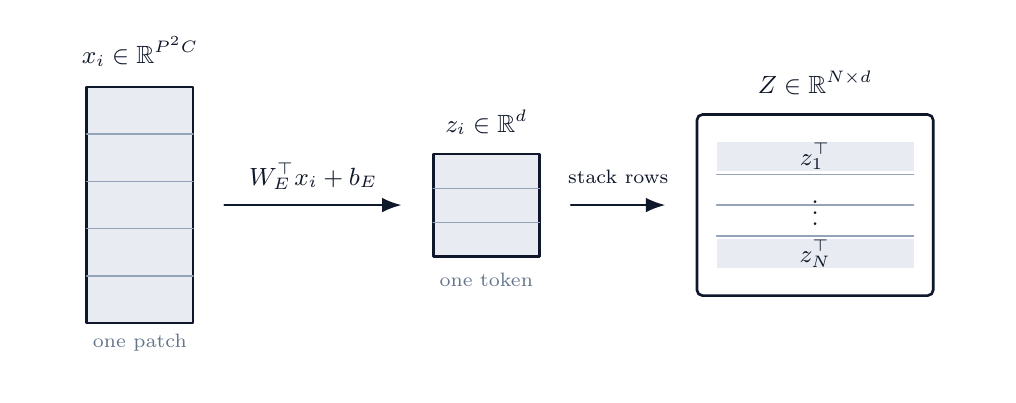
\begin{tikzpicture}[
  font=\sffamily,
  >=Latex,
  line cap=round,
  line join=round
]
  \fill[white] (-0.75,-0.65) rectangle (11.45,3.75);

  % One flattened patch represented as a column vector.
  \draw[ink, line width=0.95pt, fill=highlight!45]
    (0,0) rectangle (1.35,3.0);
  \draw[gridline, line width=0.55pt] (0,0.6) -- (1.35,0.6);
  \draw[gridline, line width=0.55pt] (0,1.2) -- (1.35,1.2);
  \draw[gridline, line width=0.55pt] (0,1.8) -- (1.35,1.8);
  \draw[gridline, line width=0.55pt] (0,2.4) -- (1.35,2.4);
  \node[ink, font=\small] at (0.675,3.45)
    {$x_i \in \mathbb{R}^{P^2C}$};
  \node[muted, font=\scriptsize] at (0.675,-0.25)
    {one patch};

  % The learned linear projection creates one d-dimensional token.
  \draw[ink, ->, line width=0.9pt]
    (1.75,1.5) -- (4.0,1.5)
    node[midway, above=4pt, fill=white, inner sep=1pt, font=\small]
      {$W_E^\top x_i + b_E$};

  \draw[ink, line width=0.95pt, fill=highlight!45]
    (4.4,0.85) rectangle (5.75,2.15);
  \draw[gridline, line width=0.55pt] (4.4,1.28) -- (5.75,1.28);
  \draw[gridline, line width=0.55pt] (4.4,1.71) -- (5.75,1.71);
  \node[ink, font=\small] at (5.075,2.55)
    {$z_i \in \mathbb{R}^{d}$};
  \node[muted, font=\scriptsize] at (5.075,0.55)
    {one token};

  % The token rows are stacked into the matrix Z.
  \draw[ink, ->, line width=0.9pt]
    (6.15,1.5) -- (7.35,1.5)
    node[midway, above=6pt, fill=white, inner sep=1.5pt, font=\scriptsize]
      {stack rows};

  \draw[ink, line width=0.95pt, rounded corners=2pt]
    (7.75,0.35) rectangle (10.75,2.65);
  \fill[highlight!45] (8.0,1.93) rectangle (10.5,2.3);
  \fill[highlight!45] (8.0,0.7) rectangle (10.5,1.07);
  \draw[gridline, line width=0.55pt] (8.0,1.5) -- (10.5,1.5);
  \draw[gridline, line width=0.55pt] (8.0,1.11) -- (10.5,1.11);
  \draw[gridline, line width=0.55pt] (8.0,1.89) -- (10.5,1.89);
  \node[ink, font=\small] at (9.25,3.05)
    {$Z \in \mathbb{R}^{N\times d}$};
  \node[ink, font=\small] at (9.25,2.12) {$z_1^\top$};
  \node[ink, font=\small] at (9.25,1.5) {$\vdots$};
  \node[ink, font=\small] at (9.25,0.88) {$z_N^\top$};
\end{tikzpicture}
\end{document}
